%% Sprach Modell
\subsection{Uebersicht und Anwendungsbereich eines Sprach-Modells}


\begin{figure}[htbp]
%\centering
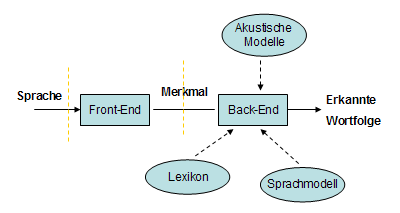
\includegraphics[width=3.5in]{Images/spracherkennungsystem}
\caption{\label{spracherkennungsystem}Aufbau eines Spracherkenungssystems}
\end{figure}
%Besteht aus  Front-und Back-End Sprache 
%Im Front wird die akusitische Merkmale eines sSprachesignals extrakiert
%Im Back-End 
%Sprachemodell: Sytaktische und semantische Einschraenkung der moeglichen Wortfolgen
%Akusitisches Modell. Statische Modelle fuer Spracheuntereinheiten(z.B.Phoneme/Triphone)
%Lexikon: Moeglichen Woeter und ihre phonetische Transkription


Was ist ein Sprachmodell? 
Wahrscheinlichkeit Woeter $p$ ($w$) oder Wortfolgen $p$ $w$.
%ein Sprachmodell wird durch die Wahrscheinlichkeit Woeter oder Wortfolgen angegeben.
\subsection{M-Gram}
\subsection{Discount}
\subsection{Back-off}